% LTeX: language=en-GB
%Author(s), Course variables
\newcommand{\titl}{02132 Assignment 3 report}
\newcommand{\subtitl}{Implementation of an FSMD-based hardware\\accelerator for the image erosion in Chisel}
\newcommand{\authone}{Niclas Juul Schæffer}
\newcommand{\SIDone}{s224744}
\newcommand{\authtwo}{Rasmus Kronborg Finnemann Wiuff}
\newcommand{\SIDtwo}{s163977}
\newcommand{\lb}{\\}
%Basics
\documentclass[a4paper, english]{article}
\usepackage[utf8]{inputenc}
\usepackage[T1]{fontenc}
\usepackage[bitstream-charter]{mathdesign}
\usepackage{babel}
\usepackage[moderate, mathspacing=normal]{savetrees}
%Symbols and scientifics
\usepackage{bm}
\usepackage{physics}
\usepackage{mathtools}
\numberwithin{equation}{section}
\usepackage{siunitx}
\sisetup{
per-mode = power ,
round-mode = figures ,
round-precision = 3 ,
exponent-mode = input ,
output-decimal-marker = {.} ,
exponent-product = 	imes ,
uncertainty-mode = separate ,
range-phrase = - ,
range-units =  single ,
inter-unit-product = \ensuremath{{\cdot{}}} ,
quantity-product = \ ,
separate-uncertainty-units = single ,
}

%Appendix, TOC and Bibliography
\usepackage{appendix}
\renewcommand\appendixtocname{Appendix}
\usepackage[nottoc]{tocbibind}
\setcounter{tocdepth}{2}
\usepackage{lastpage}

%Figures
\usepackage[svgnames]{xcolor} % Required to specify font color
\usepackage{float}
\usepackage{graphicx}
\usepackage{subcaption}
\usepackage[format=plain,
    labelfont={bf,it,footnotesize},
    textfont={it,footnotesize}]{caption}
% \captionsetup[table]{name=Huskeord}
\captionsetup{font={stretch=0.9}}
\usepackage{wrapfig}
\usepackage[a4paper, centering, rmargin=2.5cm, tmargin=2.5cm, lmargin=2.5cm, bmargin=3.5cm]{geometry}
\usepackage{verbatim}
\usepackage[space]{grffile}
\usepackage[final]{pdfpages}
\usepackage{pdflscape}
\usepackage{multirow}
\usepackage{fontawesome}
\usepackage{tikz}
% \usetikzlibrary{external}
% \tikzexternalize[prefix=tikz/]
\usepackage{circuitikz}
\ctikzset{logic ports = ieee}
\usetikzlibrary{positioning,arrows,automata}
\newcommand{\pin}[3]{\node[blue, font = \small, #2] at (#1) {#3};
                     \coordinate (#3) at (#1);}
\newcommand{\port}[4]{\node[circ, #2] (#1) {};
                     \node[#3] at (#1) {#4};}
%Header footer
\usepackage{fancyhdr}
\pagestyle{fancy}
\lhead{02132 Computer Systems \lb Assignment 3 \lb December \nth{1}}
\chead{
\includegraphics[width=.05\textwidth]{DTU}}
\rhead{Group 22 \lb \authone \ \textbf{\SIDone} \lb \authtwo \ \textbf{\SIDtwo}}
\cfoot{Page \thepage\, of\, \pageref*{LastPage}}
\renewcommand{\headrulewidth}{0.4pt}
\renewcommand{\footrulewidth}{0.4pt}
\setlength{\headheight}{36.75034pt}

%Text tools
\usepackage{listings}
\usepackage{parcolumns}
\usepackage[super]{nth}
\usepackage[normalem]{ulem}
\usepackage{import}
\usepackage{url}
\usepackage{lipsum}
\usepackage{microtype}
\usepackage[pdfencoding=auto, psdextra]{hyperref}
\hypersetup{
    colorlinks   = true, %Colours links instead of ugly boxes
    urlcolor     = blue, %Colour for external hyperlinks
    linkcolor    = blue, %Colour of internal links
    citecolor   = red %Colour of citations
}
\usepackage[capitalise]{cleveref}
% \crefname{table}{Huskeord}{Huskeord}
\usepackage{enumitem}
\newlist{arrowlist}{itemize}{1}
\setlist[arrowlist]{label={\(\rightarrow\)}}
\usepackage{tabularray}
\UseTblrLibrary{booktabs}
\usepackage{todonotes}
\usepackage[square, longnamesfirst, numbers]{natbib}
\usepackage{empheq}
% % \usepackage[newfloat, outputdir=/]{minted} % Overleaf minted buildpath fix
% \usepackage[newfloat]{minted}
% \setminted{fontsize=\small,
%            linenos=true}
% \usemintedstyle{tango}
% \SetupFloatingEnvironment{listing}{listname=Listings}
% \captionsetup[listing]{position=top, skip=-1pt}
% \newcommand{\im}[3]{\inputminted[linenos=true, python3=true, firstline=#2, lastline=#3]{python}{#1}}
% \newcommand{\java}[3]{\inputminted[linenos=true, firstline=#2, lastline=#3]{java}{#1}}
% \usepackage{dirtree}

%Definitions and new commands
\newcommand{\degr}{^{\circ}}
\newcommand{\me}{\mathrm{e}}

%Title and sectioning
\def\Vhrulefill{\leavevmode\leaders\hrule height 0.7ex depth \dimexpr0.4pt-0.7ex\hfill\kern0pt}
\usepackage{titlesec}
\usepackage{titling}
\definecolor{DTUred}{cmyk}{0, .91, .72, .23}
\definecolor{FMNgrey}{cmyk}{.73,.43,.53,.38}
%Use letters insted of numbers in section numbering
% \renewcommand{\thesection}{\Alph{section}}
% \renewcommand{\thesubsection}{\Alph{subsection}}

\makeatletter
\newcommand{\github}[1]{%
   \href{#1}{\color{DTUred}\faGithub}%
}
\makeatother

\begin{document}

\titleformat{\section}[block]
{\normalfont\Large\scshape\filright\color{DTUred}}{\fbox{\thesection}}{1em}{}

\titleformat{\subsection}
{\titlerule
    \vspace{.8ex}%
    \normalfont\scshape\color{FMNgrey}}
{\thesubsection.}{.5em}{}

\titleformat{\subsubsection}[wrap]
{\normalfont\fontseries{b}\selectfont\filright}
{\thesubsubsection.}{.5em}{}
\titlespacing{\subsubsection}
{12pc}{1.5ex plus .1ex minus .2ex}{1pc}

\title{\vspace{-40mm}\Huge\scshape\color{DTUred} \titl\lb\vspace{-4mm}\rule{4cm}{0.5mm}\lb\Large{\subtitl}}
\date{December \nth{1}}
\preauthor{\begin{center}
        \large \lineskip 0.5em%
        \begin{tabular}[t]{r}}
            \author{\textbf{Group: 22} \lb \lb \authone \ \textbf{\SIDone} \lb \authtwo \ \textbf{\SIDtwo} \lb \href{https://github.com/rwiuff/02132Assignment3}{\color{DTUred}github.com/rwiuff/02132Assignment3} \github{https://github.com/rwiuff/02132Assignment3}}
            \postauthor{\end{tabular}\par\end{center}}
\maketitle

\pagenumbering{arabic}

\thispagestyle{empty}

\section{Work distribution}
\cref{tbl:ansvar} shows the work distribution for this project.
\begin{table}[H]
    \centering
    \caption{Work distribution on the project}\label{tbl:ansvar}
    \begin{tabular}{lll}
        \toprule
        Name                 & Development tasks & Report tasks \\
        \midrule
        Niclas Juul Schæffer &                   &              \\
        \midrule
        Rasmus Wiuff         &                   &              \\
        \bottomrule
    \end{tabular}
\end{table}
\section{Design}
% \textit{Explain here what the design process was. Show the state diagram of the FSMD and explain and motivate you design decisions.}
First a CFG was generated from the pseudocode in the assignment material, yielding the graph in \cref{fig:cfg}.
\begin{figure}[H]
    \centering
    \caption{Control flow graph of erosion algorithm}\label{fig:cfg}
    \begin{tikzpicture}[
            roundnode/.style={rectangle, rounded corners=3mm, draw=black, fill={rgb:black,1;white,10}, very thick, minimum size=8mm},
            squarednode/.style={rectangle, rounded corners=3mm, draw=black!60, fill={rgb:black,1;white,10}, very thick, minimum size=8mm},
        ]
        \node[squarednode]  (start)                                         {\texttt{Start}};
        \node[roundnode]    (init)   [right = .5 of start, align = center]  {\texttt{x = 0}\\\texttt{y = 0}};
        \node[roundnode]    (checkX) [below = .5 of init]                   {\texttt{x < 19}};
        \node[squarednode]  (done)   [left = .5 of checkX]                  {\texttt{Done}};
        \node[roundnode]    (incX)   [below = .5 of checkX, align = center] {\texttt{y = 0}\\\texttt{x++}};
        \node[roundnode]    (checkY) [right = .5 of incX]                   {\texttt{y < 19}};
        \node[roundnode]    (x0)     [below = .5 of checkY]                 {\texttt{if x == 0}};
        \node[roundnode]    (x19)    [below = .5 of x0]                     {\texttt{if x == 19}};
        \node[roundnode]    (y0)     [below = .5 of x19]                    {\texttt{if y == 0}};
        \node[roundnode]    (y19)    [below = .5 of y0]                     {\texttt{if y == 19}};
        \node[roundnode]    (inner)  [below = .5 of y19]                    {\texttt{if in\_image(x,y) == 0}};
        \node[roundnode]    (erode)  [right = .5 of y0]                     {\texttt{out\_image(x,y) = 0}};
        \node[roundnode]    (incY)   [right = .5 of checkY]                 {\texttt{y++}};
        \node[roundnode]    (or)     [right = .5 of erode, align = right]   {\texttt{if in\_image(x-1,y) == 0}\\\texttt{|| in\_image(x+1,y) == 0}\\\texttt{|| in\_image(x,y-1) == 0}\\\texttt{|| in\_image(x,y+1) == 0}};
        \node[roundnode]    (skip)   at (incY -| or)                        {\texttt{out\_image(x,y) = 255}};
        \draw[->] (start.east) -- (init.west);
        \draw[->] (init.south) -- (checkX.north);
        \draw[->] (checkX.west) -- (done.east);
        \draw[->] (checkX.east) -| (checkY.north);
        \draw[->] (checkY.west) -- (incX.east);
        \draw[->] (incX.north) -- (checkX.south);
        \draw[->] (checkY.south) -- (x0.north);
        \draw[->] (x0.south) -- (x19.north);
        \draw[->] (x19.south) -- (y0.north);
        \draw[->] (y0.south) -- (y19.north);
        \draw[->] (y19.south) -- (inner.north);
        \draw[->] (inner.south) -- ++(0,-.5) -| (or.south);
        \draw[->] (x0.east) -| (erode.north);
        \draw[->] (x19.east) -- (erode.north west);
        \draw[->] (y0.east) -- (erode.west);
        \draw[->] (y19.east) -- (erode.south west);
        \draw[->] (inner.east) -| (erode.south);
        \draw[->] (or.west) -- (erode.east);
        \draw[->] (or.north) -- (skip.south);
        \draw[->] (erode.north east) ++(-1,0) -- ++(0,3) -| (incY.south);
        \draw[->] (skip.west) -- (incY.east);
        \draw[->] (incY.west) -- (checkY);
    \end{tikzpicture}
\end{figure}
This gives a good idea of the needed states in the FSMD. On the getgo two obvious optimisations can be done here. The y incrementor is constant with both writing operations, and can be split into these. We also see that the bordercases could be replaced by a single state using a more complex logical ciruit. The inner pixel check can also be merged into this state as it is still on the same control path and leads to the zerorising of the output pixel or the check for neighbouring pixels.\newline
\cref{fig:fsmd} shows the state diagram.
\begin{figure}[H]
    \centering
    \caption{State diagram of the erosion accelerator FSMD}\label{fig:fsmd}
    \resizebox{\textwidth}{!}{%
        \begin{tikzpicture}[shorten >=1pt,node distance=2cm,on grid,auto]
            \tikzstyle{every state}=[fill={rgb:black,1;white,10}]
            \node[state, initial, accepting] (idle)                           {idle};
            \node[state]                     (reginit) [right = 5 of idle]    {regInit};
            \node[state]                     (count)   [below = 3 of reginit] {count};
            \node[state, align=left]         (regup)   [left = 6 of count]    {reg\\Update};
            \node[state]                     (done)    [right = 4 of count]   {done};
            \node[state, align=left]         (check)   [below = 4 of done]    {check\\Pixel};
            \node[state]                     (write)   [below = 5 of count]   {write};

            \path[->]
            (idle)    edge [loop above] node                           {\textbf{start == 0} / \_}          ( )
            (done)    edge [loop above] node                           {\textbf{True} / done = 1}          ( )
            (idle)    edge              node                           {\textbf{start == 1} / varReg = 20} (reginit)
            (reginit) edge [loop right] node                           {\textbf{varReg < 60} / varReg++}   ( )
            (reginit) edge              node[right, align=right]       {\textbf{varReg == 60}}             (count)
            (count)   edge [bend right] node[above]                    {\textbf{xReg == 20}}               (regup)
            (regup)   edge [bend right] node[below, align=right]       {\textbf{varReg == 60} / yReg++ \\
                    xReg = 0}                          (count)
            (regup)   edge [loop above] node                           {\textbf{varReg < 60} / varReg++}   ( )
            (count)   edge [bend left]  node[right, align=right]       {\textbf{xReg < 20} / addressReg = \\
                    \(x + 20 \times y + 400\)}         (check)
            (count)   edge [bend right] node[below left, align=right]  {\textbf{xReg == 0 || xReg == 19}\\
                    \textbf{|| yReg == 0 || yReg == 19}\\
                    / addressReg=\\
                    \(x + 20 \times y + 400\)
                    \\dataWrite = 0}                   (write)
            (check)   edge [bend left]  node[below, align=right]       {\textbf{False} / dataWrite = 255}  (write)
            (check)   edge [bend right] node[above, align=right]       {\textbf{True} / dataWrite = 0}     (write)
            (write)   edge              node[right]                    {xReg++}                            (count)
            (count)   edge              node                           {\textbf{yReg == 20}}               (done)
            ;
        \end{tikzpicture}
    }%
\end{figure}
A list of registers are used to reduce read/write operations to/from the memory. The idea is to store three rows at a time, as to satisfy the erosion mask. On every iteration only one row is loaded into the register. The Register scheme is seen in \cref{fig:regs}.
\begin{figure}[H]
    \centering
    \caption{The registers in the accelerator}\label{fig:regs}
    \resizebox{.7\textwidth}{!}{%
        \begin{tikzpicture}
            \draw[black, very thick]   (0,0)    rectangle (3,3);
            \draw[step=1.0,black,thin] (0,0)    grid      (3,3);
            \draw[black, very thick]   (4,0)    rectangle (6,3);
            \draw[step=1.0,black,thin] (4,0)    grid      (6,3);

            \draw[black, very thick]   (6.5,2)  rectangle (7.5,3);
            \draw[black, very thick]   (6.5,.5) rectangle (7.5,1.5);
            \draw[black, very thick]   (8,2)    rectangle (10,3);
            \draw[black, very thick]   (8,.5)   rectangle (10,1.5);

            \node (x)     at (7,2.5)   {xReg};
            \node (y)     at (7,1)     {yReg};
            \node (reg)   at (9,2.5)   {addressReg};
            \node (inc)   at (9,1)     {varReg};

            \node (R0)    at (.5,2.5)  {R0};
            \node (R1)    at (1.5,2.5) {R1};
            \node (R2)    at (2.5,2.5) {R2};
            \node (dots1) at (3.5,2.5) {\(\cdots\)};
            \node (R18)   at (4.5,2.5) {R18};
            \node (R19)   at (5.5,2.5) {R19};

            \node (R20)   at (.5,1.5)  {R20};
            \node (R21)   at (1.5,1.5) {R21};
            \node (R22)   at (2.5,1.5) {R22};
            \node (dots2) at (3.5,1.5) {\(\cdots\)};
            \node (R38)   at (4.5,1.5) {R38};
            \node (R39)   at (5.5,1.5) {R39};

            \node (R40)   at (.5,.5)   {R40};
            \node (R41)   at (1.5,.5)  {R41};
            \node (R42)   at (2.5,.5)  {R42};
            \node (dots3) at (3.5,.5)  {\(\cdots\)};
            \node (R58)   at (4.5,.5)  {R58};
            \node (R59)   at (5.5,.5)  {R59};
        \end{tikzpicture}
    }%
\end{figure}
Furthermore registers are needed to store the memory address, the x and the y counters and a variable register to help with data register management. The state \texttt{regInit} initialises the data registers by filling R20-R59. The top row needs to be set to zero anyway. On every iteration the registers are updated as shown in \cref{fig:update}.
\begin{figure}[H]
    \centering
    \caption{Data register update}\label{fig:update}
    \begin{subfigure}[t]{.35\textwidth}
        \caption{Image rows move up}\label{fig:update1}
        \resizebox{\textwidth}{!}{%
            \begin{tikzpicture}
                \draw[black, very thick]   (0,0) rectangle (4,3);
                \draw[step=1.0,black,thin] (0,0) grid      (4,3);

                \draw[black, very thick]   (0,-2) rectangle (4,-1);
                \draw[step=1.0,black,thin] (0,-2) grid      (4,-1);

                \node (R0)    at (.5,2.5)  {R0};
                \node (R1)    at (1.5,2.5) {R1};
                \node (R2)    at (2.5,2.5) {R2};
                \node (dots1) at (3.5,2.5) {\(\cdots\)};

                \node (R20)   at (.5,1.5)  {R20};
                \node (R21)   at (1.5,1.5) {R21};
                \node (R22)   at (2.5,1.5) {R22};
                \node (dots2) at (3.5,1.5) {\(\cdots\)};

                \node (R40)   at (.5,.5)   {R40};
                \node (R41)   at (1.5,.5)  {R41};
                \node (R42)   at (2.5,.5)  {R42};
                \node (dots3) at (3.5,.5)  {\(\cdots\)};

                \node (mem1)  at (.5,-1.5)  {\small M(x,y)};
                \node (mem2)  at (1.5,-1.5) {\small M(x,y)};
                \node (mem3)  at (2.5,-1.5) {\small M(x,y)};
                \node (dots4) at (3.5,-1.5) {\(\cdots\)};

                \path[->]
                (R20) edge [bend right] (R0)
                (R21) edge [bend right] (R1)
                (R22) edge [bend right] (R2)
                (R40) edge [bend right] (R20)
                (R41) edge [bend right] (R21)
                (R42) edge [bend right] (R22);
            \end{tikzpicture}
        }%
    \end{subfigure}
    \hspace{5em}
    \begin{subfigure}[t]{.35\textwidth}
        \caption{New image row from memory}\label{fig:update2}
        \resizebox{\textwidth}{!}{%
            \begin{tikzpicture}
                \draw[black, very thick]   (0,0)  rectangle (4,3);
                \draw[step=1.0,black,thin] (0,0)  grid      (4,3);

                \draw[black, very thick]   (0,-2) rectangle (4,-1);
                \draw[step=1.0,black,thin] (0,-2) grid      (4,-1);

                \node (R0)    at (.5,2.5)   {R0};
                \node (R1)    at (1.5,2.5)  {R1};
                \node (R2)    at (2.5,2.5)  {R2};
                \node (dots1) at (3.5,2.5)  {\(\cdots\)};

                \node (R20)   at (.5,1.5)   {R20};
                \node (R21)   at (1.5,1.5)  {R21};
                \node (R22)   at (2.5,1.5)  {R22};
                \node (dots2) at (3.5,1.5)  {\(\cdots\)};

                \node (R40)   at (.5,.5)    {R40};
                \node (R41)   at (1.5,.5)   {R41};
                \node (R42)   at (2.5,.5)   {R42};
                \node (dots3) at (3.5,.5)   {\(\cdots\)};

                \node (mem1)  at (.5,-1.5)  {\small M(x,y)};
                \node (mem2)  at (1.5,-1.5) {\small M(x,y)};
                \node (mem3)  at (2.5,-1.5) {\small M(x,y)};
                \node (dots4) at (3.5,-1.5) {\(\cdots\)};

                \path[->]
                (mem1) edge [bend right] (R40)
                (mem2) edge [bend right] (R41)
                (mem3) edge [bend right] (R42);
            \end{tikzpicture}
        }%
    \end{subfigure}
\end{figure}
\section{Implementation}
\textit{Briefly discuss the implementation in Chisel of your design. You can include some code snippets if these are relevant to explain certain aspects of the implementation. In other words, try to answer the question ``What does a reader need to know about your Chisel implementation?''}
\section{Test And Evaluation}
\textit{Report here the results from the test you have carried out. Present how you have tested (paper and pencil testing) the FSMD you have designed. Present the tests you have developed (if any). Remember to discuss the relusts and the test you have carried out, do not just present them, but explain and argue their meaning. Adress the design evaluation questions in Task 6 in the Assignment 3 document.}
% \section{References}
% \begin{thebibliography}{1}
%     \bibitem{arduino}
%     Arduino, José Bagur, Taddy Chung \emph{Arduino Memory Guide (19/09/2023)\newline \href{https://docs.arduino.cc/learn/programming/memory-guide}{https://docs.arduino.cc/learn/programming/memory-guide}}
% \end{thebibliography}
%Bibliography herunder:
%\newpage

%\bibliographystyle{unsrtnat}
%\bibliography{Bibliography}

%\newpage

%\listoffigures
% \newpage
% \listoftables
%\newpage

%Appendicer herunder:

%\input{Appendix.tex}

\end{document}